% !TeX spellcheck = da_DK
\section{Behandling af biologiske signaler}
Et biologisk signal skal behandles for at kunne give feedback til patienten samt et digitalt output evt. til plejepersonale. For at kunne behandle et signal fra et accelerometer kræves der bl.a. forstærkning, filtrering, komparator samt ADC. Der kan anvendes andre komponenter til signalbehandling ift. hvad accelerometret skal benyttes til, men de nævnte vil blive benyttet i dette projekt. 

\subsection{Forstærker}\label{forstaerkerafsnit}
En forstærker kan benyttes til at ændre inputtet i form af et biologisk signal til et skaleret output. Dette kan gøres ved at kombinere en operationsforstærker med modstande, der derved kan skalere, invertere, addere og subtrahere signalet. Der findes fire forskellige forstærkningskredsløb til at udføre de nævnte opgaver: \cite{Nilsson2011}
\begin{itemize}
\item Inverterende forstærkningskredsløb: Benyttes til at invertere signalet samtidig med det skaleres.% Inverteringen af signalet betyder, at der ændres fortegn på signalet.
\item Summerende forstærkningskredsløb: Fungerer ligesom det inverterende forstærkningskredsløb med den undtagelse, at inputsignalerne summeres.
\item Ikke-inverterende forstærkningskredsløb: Benyttes til at skalere input signalet.
\item Differens forstærkningskredsløb: Benyttes til at trække to input signaler fra hinanden, så outputsignalet bliver forskellen på de to inputsignaler \cite{Nilsson2011}. Der findes forskellige typer af differensforstærkning, herunder et kredsløb med en enkelt operationsforstærker eller en instrumenteringsforstærker. I instrumenteringsforstærkeren indgår yderligere to operationsforstærkere for at lave inputbuffere til den oprindelige operationsforstærker. \cite{Sedra2010}  
\end{itemize} 

\noindent For at forstærke signalet fra et accelerometeret benyttes operationsforstærkeren, der skalerer inputspændingen til en ønsket outputspænding. Dette gøres, hvis den næste komponent skal bruge et specifikt input eller for at forstærke signaler med lav amplitude. Der kan f.eks. bruges en inverterende forstærker, som ses på \figref{invf}, hvor $V_{s}$ er det målte signal, der ønskes forstærket og $V_{o}$ er outputsignalet. Inputtets forstærkning kaldes gain og er en ratio mellem $dfrac{R_{f}}{R_{s}}$, som er de to modstande. \cite{Nilsson2011}

\begin{figure}[H]
\centering
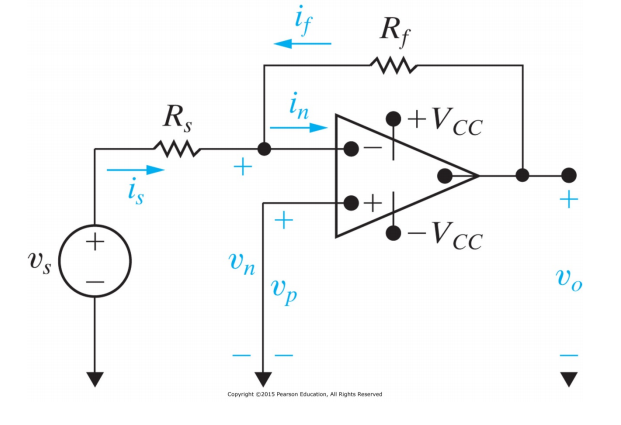
\includegraphics[scale=0.6]{figures/bProblemanalyse/inverterendeforstaerker.png}
\caption{På figuren ses en ideel operationsforstærker, som er inverterende koblet og kan forstærke input signalet $V_{s}$ til et ønsket output signal $V_{o}$ vha. modstandene $R_ {s}$ og $R_{f}$. \cite{Nilsson2011}}
\label{invf}
\end{figure}


%INDLEDE MED KORT FORKLARING PÅ HVAD EN FORSTÆRKER EGENTLIG ER OG HVILKE FORSKELLIGE TYPER DER FINDES
%UNDERSTREGE AT VI GODT VED AT DER ER FLERE FORSKELLIGE TYPER AF FORSTÆRKERE..